\setchapterpreamble[u]{\margintoc}
\glsresetall % reset glossary
\chapter{Optimizing modular structures}
Introduction
\todo{change $N_T$ con $N_\text{T}$ }
\todo{NO CELLS}
\todo{metti slend min sulle barre}
\todo{tables always small}
\section{Formulation of a modular structure optimization algorithm}
Assembled modular ultralight structures present an opportunity to greatly improve the performance and cost efficiency of modern aerostructures~\sidecite{cramer_elastic_2019}. The repetitive nature brings various interesting features among which reduced tooling, fast assembly, and short repair time. Additionally, as the mechanical performance of the structure is greatly influenced by the topology and the materials of the repetitive pattern, modular structures are naturally prone to optimization.

In the field of structure optimization, periodic materials are often modeled by means of asymptotic homogenization~\sidecite{zhou_design_2008}. The heterogeneous module topology (also called \gls{rve}) is treated as homogeneous material with associated mechanical properties \ie equivalent elastic tensor, shear modulus, etc. The homogenization approach is valid only if the \gls{rve} contains enough information about the heterogeneous material and if the structure presents significant periodicity~\sidecite{kalamkarov_asymptotic_2009,li_anisotropic_2020}. 

Nevertheless, our work pertains to structures that frequently exhibit one or more dimensions significantly smaller than the remaining dimensions, such as the thickness of a wingbox or a sandwich panel. In the context of designing modular structures (and not materials), no scale separation is assumed between the repetitive pattern and the structure itself. Consequently, the assumptions of asymptotic homogenization are not always verified. To address this, full-scale approaches~\sidecite{wu_topology_2021} have been developed.

\subsection{Variable linking}
\begin{figure*}
    \centering
    \includegraphics{figures/05_cellular_opt/00_modules_VL_bc/modules_bc.pdf}
    \caption{Notations used for the definition of the variable linking approach used to apply the modularity constraints.}
    \label{fig:05_VL}
\end{figure*}

The variable linking approach~\sidecite{zhang_scale-related_2006} is a full-scale optimization technique that involves first dividing a structure into several subdomains, which are connected in the optimization process -- \ie subdomains that belong to the same module all share the same cross-sectional areas. The primary goal is to make the manufacturing phase simpler and more efficient, allowing to assemble big structures starting from smaller repetitive modules. With this approach, the optimization perspective shifts. The optimizer design space using the variable linking approach is restricted to the optimization of the topology of the modules, using the whole structure just to evaluate and to impose the necessary mechanical constraints.

We use \figref{fig:05_VL} to illustrate the notation employed in this thesis for modular structures. On the left-hand side of the image, we have the whole test case that we aim to optimize, which is divided into $N_\text{sub}$ subdomains. Each of these subdomains is bound to exhibit the topology of one of the $N_\text{T}$ module topologies presented on the right side of the image. It is assumed for simplicity that each module has the same external shape and an identical ground structure used for discretizing the module volume. Within this framework, $\bar{n}$ represents the number of candidate bars in one module, and if we assume a fully connected mesh, we can define $\bar{n} = \bar{m} \cdot (\bar{m}-1)/2$, where $\bar{m}$ stands for the number of nodes in the module. Consequently, for the overall structure, we can write the relationship $N_{\text{el}} = N_{\text{sub}}\bar{n}$.

The vector that holds all the cross-sectional areas of the modules is represented by $\bar{\vect{a}}$, and it belongs to the set of positive real numbers $\mathbb{R}_+^{N_T \cdot \bar{n}}$. This vector is essentially a grouping of individual cross-sectional areas $\bar{\vect{a}}_t$ for each of the $N_T$ modules. In mathematical terms, $\bar{\vect{a}}$ is defined as follows:
\begin{equation}
    \bar{\vect{a}} :=  \{ \bar{\vect{a}}_t \in \mathbb{R}_+^{\bar{n}} \;|\; \forall t \in [1,\dots,N_T]\}
\end{equation}

The topology of the entire structure $\vect{a}$, which originates from the submodules' topology $\bar{\vect{a}}$, is the assembly of the individual cross-sectional areas of every one of the $N_{\text{sub}}$ subdomains and is defined as follows:
\begin{equation}
    \vect{a} :=  \{\vect{a}^j \;|\; \forall j \in [1,\dots,N_{\text{sub}}]\}
\end{equation}
and is evaluated using:
\begin{equation}
    \vect{a} = \sum_{t=1}^{N_T} \vect{h}_t\otimes\bar{\vect{a}}_t = \sum_{t=1}^{N_T} \begin{bmatrix}
        h_{1,t} \: \bar{\vect{a}}_t \\
        \vdots\\
        h_{N_{\text{sub}},t} \: \bar{\vect{a}}_t 
        \end{bmatrix}
        \label{eq:05_VL}
\end{equation}
where the $\otimes$ operator represents the Kronecher product and $\vect{h}_{t}$ is the $t$-th column of the module mapping matrix $\matr{H} = [\vect{h}_0,\dots,\vect{h}_{N_T}] \in \mathbb{B}^{N_{\text{sub}},N_T}$, where $\mathbb{B}=\lbrace 0,1 \rbrace$ is the Boolean domain. $h_{j,t}$ is the element at the $j$-th row and $t$-th column of the matrix $\matr{H}$. The module mapping matrix $\matr{H}$ indexes are defined as follows:
\marginnote{In the case of the structure shown in \figref{fig:05_VL} we have:
\begin{equation}
    \matr{H}=
\begin{bNiceMatrix}[first-row,last-col]
    \scriptstyle\textcolor{axis_gray}{t=0} &\scriptstyle\textcolor{axis_gray}{t=1}&  \\
    1 & 0 & \scriptstyle\textcolor{axis_gray}{\,j=0} \\
    1 & 0 & \scriptstyle\textcolor{axis_gray}{\,j=1} \\
    1 & 0 & \scriptstyle\textcolor{axis_gray}{\,j=2} \\
    1 & 0 & \scriptstyle\textcolor{axis_gray}{\,j=3} \\
    0 & 1 & \scriptstyle\textcolor{axis_gray}{\,j=4} \\
    0 & 1 & \scriptstyle\textcolor{axis_gray}{\,j=5} \\
    0 & 1 & \scriptstyle\textcolor{axis_gray}{\,j=6} \\
    0 & 1 & \scriptstyle\textcolor{axis_gray}{\,j=7} 
\end{bNiceMatrix}
\end{equation}
as the lower submodules (numbered from 0 to 3) exhibit the topology of module $t=0$, while the upper submodules (numbered 4 to 7) the topology of module $t=1$.}
\begin{equation}
    h_{j,t} =
    \begin{cases}
      1 & \text{if the $j$-th subdomain presents the topology of the $t$-th module,} \\
      0 & \text{otherwise.} 
    \end{cases}
\end{equation}
Lastly, we introduce some notation to denote specific bars within the modules and subdomains. We represent the cross-sectional area of the $i$-th bar of the $t$-th module as $\bar{\vect{a}}_{t,i}$, while the cross-sectional area of the $i$-th bar of the $j$-th subdomain as $\vect{a}^j_i$.
\subsection{Topological buckling of modular structures}
Addressing topological buckling in modular structures is a more complex task compared to monolithic structures. This complexity arises from the fact that we must not only consider bars within a single module's design space but also those connecting different modules. Since the nature of this problem heavily relies on how the modules are arranged within the structure, we have opted for a simplification. \marginnote{
\eqref{eq:04_chain_len}:
\begin{equation*}
    \ell^*_i(\vect{a}):= 
    \begin{cases}
        \ell_i & \text { if } i \notin \mathcal{C}_{l,r}(\vect{a}) \\
        \sum \ell_{r} \;|\; r \in \mathcal{C}_{l,r}(\vect{a})  & \text { otherwise.}
    \end{cases}
\end{equation*}
\eqref{eq:04_side_cons_chain}: 
\begin{equation*}
    a_{r}\geq a_{r=1}, \; r \in \mathcal{C}_{l,r}(\vect{a}), \; \forall r \neq 1.
\end{equation*}
} We focus only on the assessment of nodal instability within each module, modifying the length $\ell^*$ used to evaluate the critical buckling force of \eqrefnotext{eq:04_buck} and \eqref{eq:04_chain_len} only of compressive chains of bars that fall inside a module. Additionally, \eqref{eq:04_side_cons_chain} is modified as follows:
\begin{equation}\label{eq:05_side_cons_chain_modular}
    \bar{\vect{a}}_{t,r} \geq \bar{a}_{t,r=1} \quad r \in \mathcal{C}_{l,r}(\bar{\vect{a}}_t) \quad \forall t \in [1,\dots,N_T].
\end{equation}
We have made this choice knowing that the high connectivity of modular structures tends to reduce the occurrence of nodal instability within the structure. Any potential nodal instability in compressive chains at the structure level is addressed in a subsequent post-processing phase.

\subsection{Optimization formulation}
The monolithic fomulation \ref{eq:04_optim_complete} is updated using \eqsref{eq:05_VL} and \eqrefnotext{eq:05_side_cons_chain_modular} to obtain the modular optimzation formulation \ref{eq:05_optim_complete_modular} that use the variable linking approach. Formulation~\ref{eq:05_optim_complete_modular} is stated in terms of modular cross-sectional areas $\bar{\vect{a}}$, member forces $\vect{q}$ and nodal displacements $\vect{U}$ as follows:
\begin{equation}
    \begin{aligned}
    \min_{\bar{\vect{a}}, \vect{q}, \vect{U}}   && V &= \vect{\ell}^{T}\vect{a}\\
    \textrm{s.t.}  && \vect{a} &= \sum_{t=1}^{N_T} \vect{h}_t\otimes\bar{\vect{a}}_t \\ 
    && \matr{B}\vect{q} &= \vect{f} && \\
    && \vect{q} &= \frac{\vect{a}E}{\vect{\ell}}\vect{b}^T\vect{U} &&  \\
    && \vect{q} &\geq -\frac{s\vect{a}^2}{\vect{\ell}^{*2}} &&  \\
    && -\sigma_c\vect{a} &\leq \vect{q} \leq \sigma_t\vect{a} &&  \\
    && \bar{\vect{a}}_{t,r}&\geq \bar{a}_{t,r=1} && r \in \mathcal{C}_{l,r}(\bar{\vect{a}}_t),\, \forall t \\
    && 0 &\leq \bar{\vect{a}} \leq \frac{4 \pi \bar{\vect{\ell}}^2}{\lambda_{\text{max}}}, \\
    \end{aligned}
    \tag{${\mathbb{M}}_\text{1}$}
    \label{eq:05_optim_complete_modular}
\end{equation}
where $\bar{\vect{\ell}}$ represent the vector the lengths of the bars within the modules.

The total number of design variables in the formulation is expressed as $N_T\bar{n} + N_{\text{sub}}\bar{n} + 2M$ or $N_T\bar{n} + N_{\text{sub}}\bar{n} + 3M$, depending on whether the test case is two or three-dimensional. The number of constraints is, however, equal to the monolithic optimization. This fact arises due to the localized nature of stress, buckling, and compatibility constraints, which are all referenced not only to individual modules but to the entire structure.

The formulation is solved reusing the proposed two-step optimization algorithm, incorporating the reinitialization heuristic to mitigate dependence on the optimization starting point, as detailed in \secref{sec:04_2step_opt}. We state here the formulation $\mathbb{M}_\text{2}$ with relaxed compatibility constraints that is solved as the first step of the optimization. 

\begin{equation}
    \begin{aligned}
    \min_{\bar{\vect{a}}, \vect{q}, \vect{U}}   && V &= \vect{\ell}^{T}\vect{a}\\
    \textrm{s.t.}  && \vect{a} &= \sum_{t=1}^{N_T} \vect{h}_t\otimes\bar{\vect{a}}_t \\ 
    && \matr{B}\vect{q} &= \vect{f} && \\
    && \vect{q} &\geq -\frac{s\vect{a}^2}{\vect{\ell}^{*2}} &&  \\
    && -\sigma_c\vect{a} &\leq \vect{q} \leq \sigma_t\vect{a} &&  \\
    && \bar{\vect{a}}_{t,r}&\geq \bar{a}_{t,r=1} && r \in \mathcal{C}_{l,r}(\bar{\vect{a}}_t),\, \forall t \\
    && 0 &\leq \bar{\vect{a}} \leq \frac{4 \pi \bar{\vect{\ell}}^2}{\lambda_{\text{max}}}. \\
    \end{aligned}
    \tag{${\mathbb{M}}_\text{2}$}
    \label{eq:05_optim_no_constr_modular}
\end{equation}

We can solve Formulation $\mathbb{M}_2$ by breaking it down into simpler linearized problems using a \gls{slp} algorithm. This is possible because the Kronecker product is a linear operator, and the buckling constraints can be linearized, as previously demonstrated in \secref{sec:04_2step_opt}.

\subsection{Sensitivity analysis}
During each iteration of the optimization process, the current state of the structure is determined by the values assigned to the design variables. In structure optimization, the evolution of the structure's design is guided by assessing sensitivities of both the objective function and constraints with respect to the design variables. In the specific context of modular structure optimization, the module (and not the structure divided in the subdomains) is identified as the design domain, and for that reason necessitating the derivation of corresponding modular sensitivities.

The approach involves initially computing gradients for all candidates for the full monolithic structure, without considering the modularity. Subsequently, the contributions of each $i$-th bar belonging to a specific module topology $t$ are summed together. Mathematically, this can be expressed as follows:
\begin{equation}
    \derfrac{(\cdot)_i}{\bar{a}_{t,i}} =  \sum_{j=0}^{N_\text{sub}} \vect{h}_t^T \derfrac{(\cdot)_i}{a^j_i} 
    \label{eq:05_VL_grad}
\end{equation}
where $(\cdot)$ is a generic function for wich the sensitivity is calculated. This process is graphically represented in \figref{fig:05_VL_grad}.

\begin{figure*}
    \centering
    \includegraphics{figures/05_cellular_opt/00_modules_VL_grad/modules_grad.pdf}
    \caption{Notations used for the evaluation of the sensitivities for the modular structure optmization based on the variable linking scheme.}
    \label{fig:05_VL_grad}
\end{figure*}

\section{Numerical application}
In this section we formulate multiple test cases used to expmpre the limits and the carachteristics of modular structures and the proposed modular structure optimization formulation \eqrefnotext{eq:05_optim_complete_modular}.

The test cases are optimized using the two-step resolution strategy implemented with five calls of reinitialization (2S-5R) with $n_{\text{max}}=5$. The reinitialization magnitude parameter $\vect{\phi}$ is set up using the same parameters listed in \tabref{tab:05_param}, that leads to $\vect{\phi} = \left[ 0.8000, 0.6400, 0.4096, 0.1677, 0.0281 \right]$.
\begin{margintable}
        \small
    \centering
    \begin{tabular}{cc}
    \toprule
    \textbf{Parameter} & \textbf{Value} \\ \midrule
    $\phi_0$              & 0.8 \\
    $\beta$             & 2 \\
    \bottomrule
    \end{tabular}
    \caption{Reminder of the parameters used to setup the reinitialization parameters for the modular optimization. The full list of values and tolerances used for the setup of the optimization algorithm can be found in \tabref{tab:04_param}.}
    \label{tab:05_param}
\end{margintable}

The optimizations are performed using the Python package CVXPY 1.2.2 \sidecite{diamond_cvxpy_2016} with the ECOS 2.0.7 \sidecite{domahidi_ecos_2013} solver to solve the relaxed \gls{lp} Problem \eqrefnotext{eq:05_optim_no_constr_modular}. The \gls{nlp} Problem \eqrefnotext{eq:05_optim_complete_modular} is solved using cyipopt \sidecite{Moore_Mechmotum}, a Python wrapper for IPOPT 3.14.11 \sidecite{wachter_implementation_2006}, a large-scale nonlinear optimization package using PARDISO 6.0 \sidecite{alappat_recursive_2020} as linear solver. 

\subsection{On the equivalence of multi load cases and modular structures}
\begin{margintable}
    \small
    \centering
    \begin{tabular}{cc}
    \toprule
    \textbf{Parameter}        & \textbf{Value} \\ \midrule
    $L$              & 100     \\
    $E$              & 1     \\
    $\sigma_\text{c}, \sigma_\text{t}$ & $\pm 1$\\
    $P$              & 1   \\
    \bottomrule
    \end{tabular}
    \caption{Material data used for the modular bridge section 2D structure.}
    \label{tab:05_modular_data}
\end{margintable}
The first test case we deal with is a two-dimensional bridge structure segment composed of two subdomains ($n_{\text{sub}} = 2$) with symmetric boundary conditions, as illustrated in \figref{fig:05_cell_multi_eq_bcs}a. In this test case, two vertical loads of magnitude P=1 are applied to the lower side of the design space. The material and geometrical details are given in \tabref{tab:05_modular_data} and are normalized and adimensional for simplicity. Each subdomain of the structure is discretized using a 15x15 fully connected ground structure, with a number of candidates $\bar{n}=$ per subdomain. It is important to note that, for this example, buckling constraints have been deactivated.

Additionally, a similar structure is optimized, comprising only a single submodule, subjected to two distinct load cases, denoted as $p_1$ and $p_2." These loads are positioned at precisely the same distance from the support, as illustrated in Figure xx b.
\todo{table results}
\begin{figure}[]
    \hspace*{\fill}
    \subcaptionbox{}{\includegraphics[height=4.15cm]{figures/05_cellular_opt/00_cell_multi_eq_bcs/cell_bcs.pdf}}
    \hfill
    \subcaptionbox{}{\includegraphics[height=4.15cm]{figures/05_cellular_opt/00_cell_multi_eq_bcs/multiload_bcs.pdf}}
    \hspace*{\fill}
    \caption{}
    \label{fig:05_cell_multi_eq_bcs}
\end{figure}


\begin{table}
    \centering
    \small
    \begin{tabular}{lcc}
        \toprule
        \textbf{Quantity} & Multi-subdomain & Multi-loads \\ \midrule
    $N_\text{sub}$       &1& 2   \\
    $N_\text{opt}\;(N_\text{el})$ & 31 (25200)& 62 (50400) \\
    $V$ & 91.346 & 182.692  \\ \bottomrule
    \end{tabular}
    \caption{}
    \label{tab:05_}
    \end{table}

we optimized the two load cases using p = 0.05 for the first case and p = 0.1 for the second. we get exactly the same topology with vol V1 = 2V2. this simple example mette in luce an interesting property of the optimization of modular structures that could have been theorized only using common sense. when a loaded structure is subdivided in multiple subdomains, every one subdomain, if isolated from the sturcture and apllying the correct boundary conditions made by the reaction forces of the adjacent bars and supports, is subject to different loading conditions. if then we apply some modularity constarints to all of these modules, we are looking for the best structure that optimize contemporanely all of these different load cases.

\begin{figure}[]
    \hspace*{\fill}
    \subcaptionbox{}{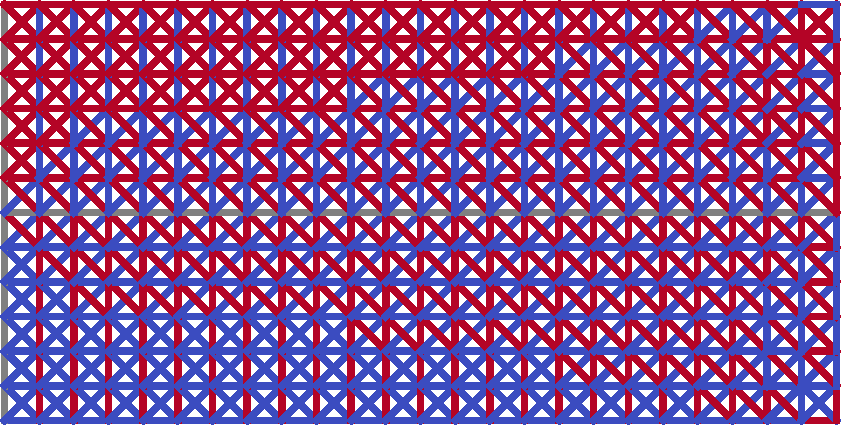
\includegraphics[height=3.5cm]{figures/05_cellular_opt/00_cell_multi_equivalence/cell.pdf}}
    \hfill
    \subcaptionbox{}{\includegraphics[height=3.5cm]{figures/05_cellular_opt/00_cell_multi_equivalence/multiload.pdf}}
    \hspace*{\fill}
    \caption{\todo{spiega colori as usual}}
    \label{fig:05_cell_multi_eq}
\end{figure}
Furthermore, this examples confirm us that when dealing with modularity constraints, we need to solve the quindi conferma del bisogno di usare l nlp con i kinematic constraints

\subsection{Parametric study on the number of subdomains and the complexity of the module}

\begin{marginfigure}
    \centering
    \includegraphics[width=\linewidth]{figures/05_cellular_opt/00_supported_bc/supported_3D_symm.pdf}
    \caption{In gray the symmetry planes.}
    \label{fig:05_symm_support_bc}
\end{marginfigure}
\begin{margintable}
    \small
    \centering
    \begin{tabular}{cc}
    \toprule
    \textbf{Parameter}        & \textbf{Value} \\ \midrule
    $E$              & \qty{2.7}{GPa}     \\
    $\nu$            & 0.3   \\
    $\sigma_\text{c}, \sigma_\text{t}$ & $\pm $\qty{55}{MPa} \\
    $\rho$              & \qty{1.14}{\gram\per\cubic\centi\metre}   \\
    $P$              & \qty{100}{N}   \\
    \bottomrule
    \end{tabular}
    \caption{Material data used for the simply supported 3D beam optimization.}
    \label{tab:05_3D_supp_mat}
\end{margintable}
\begin{marginfigure}
    \centering
    \includegraphics[width=\linewidth]{figures/04_TTO_improvements/16_supported_3D_sol/04_Topology_NLP_iso-min.png}
    \caption{with a vol of}
    \label{fig:05}
\end{marginfigure}
We conduct here a parametric study on the 3d supported truss already treated in monolithic in section xx. in this study we limit to one single module Nt=1 and we do not study yet the effect that it has to have multiple module topologies on the optimized structure. additionally we limit to cubic cell shape. we do a recap of the loading case and the geometric and material properties in table and in \figref{fig:05_symm_support_bc}.
\todo{number of subdomains and not subdomain number}

we propose here two new metrics used to better understand how the modular structures are loaded. The first one is called structural efficency index $\varphi$ that we will use to quickly assesshow many bars are used approaching the fully stressed state described by Michell \sidecite{michell_limits_1904}. it is defined as :
\begin{equation}
    \varphi = \frac{N_\text{opt,f}\times100}{N_\text{opt}}
\end{equation}
where $N_\text{opt,f}$ is the number of bars that activate either the tensile stress, the compressive stress, or the buckling constraints, defined as follows:
\begin{equation}
    N_\text{opt,f} = \operatorname{card}(\{i\;|\;c_\text{f,i} > 0.95\})
\end{equation}
where $\vect{c}_\text{f}=\max{\left(-\vect{q} /\sigma_c \vect{a},\:\vect{q} /\sigma_t \vect{a},\:\vect{q}/\vect{q}_{\text{crit}}\right)}$ represent the normalized mechanical failure criterion and $\operatorname{card}(\{\cdot\})$ represent the cardinality of the set $\{\cdot\}$.

The second metric is $\psi$ and is defined as the mean value of the normalized mechanical failure criterion $\vect{c}_\text{f}$ weighted on the volumes of the individual bars $\vect{v}$:
\begin{equation}
    \psi = \frac{1}{V} \left( \sum_{i=0}^{N_\text{opt}} v_i c_\text{f,i} \right)
\end{equation}

This parameter is comprised betweent 0 and 1 and the more is near one the more the bars are averagely near a the upper bound of one of the mechanical failure constrants. major importance is given to more voluminoous bars.

\paragraph{Influence of the number of the subdomains}
We first study the influence of the number (and consequently the scale, we use here the two terms indistinguibely) of the subdomains in the structure. the structure is divided in a different number of cubic and equals subdomqins, while the test case and the material will be still the same. The entire structure is divided in 6x2x3, 12x4x6,18x6x9, and 30x10x15 submodules in the X, Y, and Z axis and every subdomain is discretized by a 2x2x2 fully connected ground structure with nbar=28. The very same thest is conducted also on a 3x3x3 fully connected ground structure with nbar=351 to be sure that the trends are invariant with the cell complexity.

\begin{marginfigure}
    \centering
    \includegraphics{figures/05_cellular_opt/00_module_scale_tab/scale_tab_v.pdf}
    \caption{\todo{add monolithic result with a line horizontal}}
    \label{fig:05_scale_v}
\end{marginfigure}

\begin{marginfigure}
    \centering
    \includegraphics{figures/05_cellular_opt/00_module_scale_tab/scale_tab_t.pdf}
    \caption{\todo{timel}}
    \label{fig:05_scale_t}
\end{marginfigure}

The parametric results on the influence of the number of subdomains in the structure are resumed in \tabref{tab:05_scale_results}. in there we present the numeric results toghether with a graphical representation of the module of the optimized structures for the differnet size of the repeating module. The firs important finding is that the optimized volume is very influenced by the module scale. We observe that in \figref{fig:05_scale_v}, where the volume following almost a linear relationship with respect of the number of submodules. This relationship hold even when considering 3x3x3 modules. Concerning the comutanional time, we notice that we have a similar relationship. Even if the number of variable of design remains the same, This incease is due to the increasing number of constraints (we remember that in modular optimization the mechanical constraints are evalued for every member of the structure and not of the module). Another interesting findings is that the number of active bars in the optimized module is almost not dependent of the scale of the module.

A graphical representation of the 3D structures can be observed in \figref{fig:05_scale_results}, where the isometric view, togheter with the view on the XZ planes are plotted for the case with the module with the 2x2x2 ground structure. It is really interesting to see how, when the physical dimensions of the module are high, the optimizer converge naturally towards solutions that  prioritize long tnesile members and short compressive members to comply with the local buckling constraints. However, as the size of the module shrinks (look at the 30x10x15 reusults) and with him the buckling effective length of the members, the optimized design shifts to something where tensile and compressive members are both presents. This fact is in accordance to Sigmund findings \sidecite{sigmund_non-optimality_2016}.

\begin{table*}
    \centering
    \small
    \begin{tabular}{lx{1.4cm}x{1.4cm}x{1.4cm}x{1.4cm}x{1.45cm}x{1.4cm}x{1.4cm}x{1.4cm}x{1.4cm}}
        \toprule
        \multirow{2}{*}{\textbf{Quantity}}         & 7x3x4 &\multicolumn{4}{l}{2x2x2} & \multicolumn{3}{l}{3x3x3} \\ 
             \cmidrule(lr){2-2} \cmidrule(lr){3-6} \cmidrule(lr){7-9} 
     &1x1x1& 6x2x3      & 12x4x6     &  18x6x9    &  30x10x15\textsuperscript{\emph{a}}   &   6x2x3      & 12x4x6     &  18x6x9      \\
     & -- & \includegraphics[width=1.3cm]{figures/05_cellular_opt/00_module_scale_cell/6x2x3_2x2x2_c.png}    &\includegraphics[width=1.3cm]{figures/05_cellular_opt/00_module_scale_cell/12x4x6_2x2x2_c.png}&\includegraphics[width=1.3cm]{figures/05_cellular_opt/00_module_scale_cell/18x6x9-2x2x2_c.png}&\includegraphics[width=1.3cm]{figures/05_cellular_opt/00_module_scale_cell/30x10x15-2x2x2_c.png}&\includegraphics[width=1.3cm]{figures/05_cellular_opt/00_module_scale_cell/6x2x3_3x3x3_c.png}&\includegraphics[width=1.3cm]{figures/05_cellular_opt/00_module_scale_cell/12x4x6_3x3x3_c.png}&\includegraphics[width=1.3cm]{figures/05_cellular_opt/00_module_scale_cell/18x6x9-3x3x3_c.png}        \\
    $\bar{n}_\text{opt}\;(\bar{n})$ &1984&9 (28)&9 (28) &8 (28)&8 (28)&19 (351)&15 (351)& 16 (351)\\
    $N_\text{sub}$         &1&36&288&972&4500&36&288&972  \\
    $N_\text{opt}\;(N_\text{el})$ &20 (1984)&324 (1008)&2592 (8064)&7776 (27216)&36000 (126000)&468 (12636)&4320 (101088)&  15552 (341172)       \\
    $V$ [\unit{cm^3}]&9.907&27.074&70.559&104.891&277.238&24.323&65.723&117.904         \\
    $V$ [\unit{\percent}] &1.761&4.812&12.544&18.648&49.288&4.324&11.684&20.960         \\
    C [\unit{J}]    &3.71&4.22&3.35&3.19&1.12&3.63&1.84&2.02\\
    $a_\text{max}$ [\unit{mm^2}]   &37.61&9.40&5.45&5.45&3.55&5.33&2.60&3.14         \\
    $\varphi$   &\qty{100.00}{\percent}&\qty{14.81}{\percent}&\qty{1.85}{\percent}&\qty{0.67}{\percent}&\qty{0.12}{\percent}&\qty{20.51}{\percent}&\qty{1.46}{\percent}&\qty{0.62}{\percent}         \\
    $\psi$   &1.000&0.446&0.178&0.105&0.030&0.327&0.127&0.096\\
    t     &\hms{0;0;4}&\hms{0;0;6}&\hms{0;0;48}&\hms{0;5;6}&\hms{1;17;00}&\hms{0;5;42}&\hms{0;42;50}& \hms{27;17;00} \\ \bottomrule
    \end{tabular}
    \\
    \scriptsize{\textsuperscript{\emph{a}}In this test case the minimum slenderness limit is relaxed to $\lambda_\text{max}=10$ instead of 15.}
    \caption{}
    \label{tab:05_scale_results}
    \end{table*}

    \begin{figure*}
        \hspace*{\fill}
        \subcaptionbox{}{\includegraphics[width=0.23\linewidth]{figures/05_cellular_opt/00_module_scale/6x2x3_2x2x2.png}}
        \hfill
        \subcaptionbox{}{\includegraphics[width=0.23\linewidth]{figures/05_cellular_opt/00_module_scale/12x4x6_2x2x2.png}}
        \hfill
        \subcaptionbox{}{\includegraphics[width=0.23\linewidth]{figures/05_cellular_opt/00_module_scale/18x6x9_2x2x2.png}}
        \hfill
        \subcaptionbox{}{\includegraphics[width=0.23\linewidth]{figures/05_cellular_opt/00_module_scale/30x10x15_2x2x2.png}}
        \hspace*{\fill}
        \bigskip
        \hspace*{\fill}
        \subcaptionbox{}{\includegraphics[width=0.23\linewidth]{figures/05_cellular_opt/00_module_scale/6x2x3_2x2x2_XZ.png}}
        \hfill
        \subcaptionbox{}{\includegraphics[width=0.23\linewidth]{figures/05_cellular_opt/00_module_scale/12x4x6_2x2x2_XZ.png}}
        \hfill
        \subcaptionbox{}{\includegraphics[width=0.23\linewidth]{figures/05_cellular_opt/00_module_scale/18x6x9_2x2x2_XZ.png}}
        \hfill
        \subcaptionbox{}{\includegraphics[width=0.23\linewidth]{figures/05_cellular_opt/00_module_scale/30x10x15_2x2x2_XZ.png}}
        \hspace*{\fill}
        \caption{(a-d) (e-h)}
        \label{fig:05_scale_results}
    \end{figure*}

    
    willing to undertand why the volume is so influenced by the number of submodules, we plot the allure of the parameters $\varphi$ et $\psi$ in \figref{fig:05_scale_param}. As we can see every bar of the monolithic structure activates either the buckling or the stress constraint $\varphi=\qty{100}{\percent}$ and $\psi=1$, while this is  not true for any of the modular structures. 12x4x6-3x3x3 case with many bars that stays grays.
    \begin{marginfigure}
        \centering
        \includegraphics[width=\linewidth]{figures/05_cellular_opt/00_module_scale_tab/scale_tab_param.pdf}
        \caption{\todo{timel}}
        \label{fig:05_scale_param}
    \end{marginfigure}
    
    This can be observed more clearly in \figref{fig:05_scale_failure}, where the stress and buckling constraints applied to the optimized structures of the monolithic and the 12x4x6-3x3x3 case. In this image we can see that in the 12x4x6-3x3x3 case many bars stays grays. This effect cqn be explained having a look figure xx where the stress and buckling constraints activate onlky on one submodules but force the whole structure to show it quqnd meme. the modular structure is for that reason very redundant and fail safe, but pays this in terms of total volume.
    
    \begin{figure}
        \centering
        \includegraphics[width=\linewidth]{figures/05_cellular_opt/00_module_scale_failure/12x4x6_mech.pdf}
        \caption{\todo{metti undeformed e compara con no cell}}
        \label{fig:05_scale_failure}
    \end{figure}

\paragraph{Influence of the complexity of the module}
We are now shifting our focus to another parameter of modular structures: the module complexiti, ovvero the number of candidates memeber inside a module. To understand how this parameter influence the optimized structure we set up an analysis similar to the one precedently done for the module scale. Using always the same test case, we divide the structure in 6x2x3 submodules in the X, Y, and Z axis respectively, and we discretize every module using a 2x2x2, a 3x3x3, a 4x4x4,and a 5x5x5 fully connected ground structure (nbar= nbar=). The very same thest is conducted again on a 12x4x6 structure to validate the test on a different modular structure.

\begin{table*}
    \centering
    \small
    \begin{tabular}{lx{1.4cm}x{1.4cm}x{1.4cm}x{1.4cm}x{1.4cm}x{1.4cm}x{1.4cm}x{1.4cm}}
        \toprule
        \multirow{2}{*}{\textbf{Quantity}} & \multicolumn{4}{l}{6x2x3} & \multicolumn{3}{l}{12x4x6} \\ \cmidrule(lr){2-5} \cmidrule(lr){6-8} 
     & 2x2x2      & 3x3x3     &  4x4x4    &  5x5x5    &   2x2x2      & 3x3x3        & 4x4x4      \\
     &  \includegraphics[width=1.3cm]{figures/05_cellular_opt/00_module_complexity_cell/6x2x3_2x2x2_c.png}    &  \includegraphics[width=1.3cm]{figures/05_cellular_opt/00_module_complexity_cell/6x2x3_3x3x3_c.png}    & \includegraphics[width=1.3cm]{figures/05_cellular_opt/00_module_complexity_cell/6x2x3_4x4x4_c.png}     & \includegraphics[width=1.3cm]{figures/05_cellular_opt/00_module_complexity_cell/6x2x3_5x5x5_c.png}     & \includegraphics[width=1.3cm]{figures/05_cellular_opt/00_module_complexity_cell/12x4x6_2x2x2_c.png}        & \includegraphics[width=1.3cm]{figures/05_cellular_opt/00_module_complexity_cell/12x4x6_3x3x3_c.png}   &  \includegraphics[width=1.3cm]{figures/05_cellular_opt/00_module_complexity_cell/12x4x6_4x4x4_c.png}      \\
    $\bar{n}_\text{opt}\;(\bar{n})$ &  9 (28) &   19 (351)   &  88  (2016)   &  88 (7750)    &   9 (28)   &    15 (351)        &   22   (2016)  \\
    $N_\text{sub}$           &    36  &   36   &   36   &   36   &    288     &   288      &    288    \\
    $N_\text{opt}\;(N_\text{el})$  &  324 (1008) &  468 (12636)   & 792  (72576)   & 792 (279000)     & 2592 (8064)     &   4320   (101088)       &  6336 (580608)     \\
    $V$ [\unit{cm^3}] & 27.074 & 24.323     & 17.098     & 17.083     &  70.559    &  65.723       & 60.368       \\
    $V$ [\unit{\percent}] &4.812&4.324&3.040&3.036&12.544&11.684&10.732        \\
    C [\unit{J}]      & 4.22     &   3.63   & 4.49     & 3.91     &   3.35      &  1.84       & 2.43       \\
    $a_\text{max}$ [\unit{mm^2}]      & 9.40     &   5.33   &   3.39   &  3.77    &  5.45       &   2.60      &   2.97    \\
    $\varphi$   &\qty{14.81}{\percent}&\qty{20.51}{\percent}&\qty{12.12}{\percent}&\qty{20.20}{\percent}&\qty{1.85}{\percent}&\qty{1.46}{\percent}&\qty{1.32}{\percent}         \\
    $\psi$& 0.446    &   0.327   & 0.414     & 0.419     &   0.178      &  0.127       & 0.136       \\
    t        & \hms{0;0;6}  &  \hms{0;5;42} & \hms{0;14;20} & \hms{3;17;00} & \hms{0;0;48} & \hms{0;42;50} &  \hms{32;4;00}      \\ \bottomrule
    \end{tabular}
    \caption{}
    \label{tab:05_comp_results}
    \end{table*}

The results of the parametric study are presented in a tabular way in \tabref{tab:05_comp_results}. once again we plotted the most interesting aspect in a separate plots. The first thing we look at is how the volume of the optimized structure is influenced by the module complexity. in \figref{fig:05_comp_v} we can observe tht the cell complexity has in general a beneficial effect on the volume. However the effect became less and less big the more we add complexity , and in this particular test case stagnates after 4x4x4. Concerning the comutanional time (see \figref{fig:05_comp_t}), we notice that we have a  relationship similar to the one we already observed for the subdomains scale. Even if the number of variable of design remains the same, This time the number of design variables increase with the module complexity, toghether with the increasing number of the candidates and thus the constraints. The 3d rendering of the optimized structures for the 6x2x3 case are presented in \figref{fig:05_comp_results}, in wich the reader can observe the evolution of the topology of the module toward more complex (we go from nbar active = xx to xx for the 2x2x2 and 5x5x5 case, respectively). While in the low complexity we prioritize tensile elements, in more complex we have shorter elements, less influenced by local buckling.

\begin{figure*}
    \hspace*{\fill}
    \subcaptionbox{}{\includegraphics[width=0.23\linewidth]{figures/05_cellular_opt/00_module_complexity/6x2x3_2x2x2.png}}
    \hfill
    \subcaptionbox{}{\includegraphics[width=0.23\linewidth]{figures/05_cellular_opt/00_module_complexity/6x2x3_3x3x3.png}}
    \hfill
    \subcaptionbox{}{\includegraphics[width=0.23\linewidth]{figures/05_cellular_opt/00_module_complexity/6x2x3_4x4x4.png}}
    \hfill
    \subcaptionbox{}{\includegraphics[width=0.23\linewidth]{figures/05_cellular_opt/00_module_complexity/6x2x3_5x5x5.png}}
    \hspace*{\fill}
    \bigskip
    \hspace*{\fill}
    \subcaptionbox{}{\includegraphics[width=0.23\linewidth]{figures/05_cellular_opt/00_module_complexity/6x2x3_2x2x2_XZ.png}}
    \hfill
    \subcaptionbox{}{\includegraphics[width=0.23\linewidth]{figures/05_cellular_opt/00_module_complexity/6x2x3_3x3x3_XZ.png}}
    \hfill
    \subcaptionbox{}{\includegraphics[width=0.23\linewidth]{figures/05_cellular_opt/00_module_complexity/6x2x3_4x4x4_XZ.png}}
    \hfill
    \subcaptionbox{}{\includegraphics[width=0.23\linewidth]{figures/05_cellular_opt/00_module_complexity/6x2x3_5x5x5_XZ.png}}
    \hspace*{\fill}
    \caption{(a-d) (e-h)}
    \label{fig:05_comp_results}
\end{figure*}

\begin{marginfigure}
    \centering
    \includegraphics{figures/05_cellular_opt/00_module_complexity_tab/comp_tab_v.pdf}
    \caption{\todo{add monolithic result with a line horizontal}}
    \label{fig:05_comp_v}
\end{marginfigure}

\begin{marginfigure}
    \centering
    \includegraphics{figures/05_cellular_opt/00_module_complexity_tab/comp_tab_t.pdf}
    \caption{\todo{timel}}
    \label{fig:05_comp_t}
\end{marginfigure}

\begin{marginfigure}
    \centering
    \includegraphics[width=\linewidth]{figures/05_cellular_opt/00_module_complexity_tab/comp_tab_param.pdf}
    \caption{\todo{timel}}
    \label{fig:05_comp_param}
\end{marginfigure}

It is interesting to note that the number of active bars in the optimized stucture is quite dependent on the complexity of the module. However, in this specific case we see that it saturates at 88 in the 6x2x3 case,another thing that suggest suggesting that we reached the convergence of the discretization.

Finally in \figref{fig:05_comp_param} we plot the numeric values of phi and psi. Compared to what we observed before, here So we can conclude These index helps us understanding how much a truss is charged but they don't gives us per forza some hints on the optimality : a structure that is loaded to the max of the material helps to go towards lighter design but is not sufficient, as this example show us.

\paragraph{Design of experiments}
With the data gathered until now we want to build the \gls{doe} of optimized modular structures. The goal is to monitor how the outcomes vary by introducing a change of the preconditions, which is represented by one or more independent variables. In our case the independent variables chosen are the subdomain number $N_\text{sub}$ ($x_1$) and module complexity $\bar{n}$ ($x_2$), while the response observed are the total structural volume $V$ and the computational time $t$. As done till now we limit to cubic cell for semplicity.

We decided to use a quadratic model with interaction (the term $xy$) to try to capture a possible interference between x1 and x2 as follows:
\begin{equation}
    a\:x_1^2+b\:x_2^2+c\:x_1x_2+d\:x_1+e\:x_2+f
\end{equation}
The coefficient are found solving a least squares system using the data presented before in this section.

\begin{margintable}
    \small
    \centering
    \sisetup{table-auto-round}
    \begin{tabular}{cS[table-number-alignment = center, table-format = 1.2e1]}
    \toprule
    \textbf{Coeff.} & {\textbf{Value}} \\ \midrule
    $a$ & 9.002e-08    \\
    $b$ &  -1.022e-05   \\
    $c$ &  -1.770e-06   \\
    $d$ &  -2.644e-03   \\
    $e$ &   1.011e-01  \\
    $f$ &   2.881e+01  \\
    \bottomrule
    \end{tabular}
    \caption{Volume}
    \label{tab:05_doe_coeff_v}
\end{margintable}

\begin{margintable}
    \small
    \centering
    \sisetup{table-auto-round}
    \begin{tabular}{cS[table-number-alignment = center, table-format = 1.2e1]}
    \toprule
    \textbf{Coeff.} & {\textbf{Value}} \\ \midrule
    $a$ & 1.547e-03    \\
    $b$ & -2.871e-04    \\
    $c$ &  2.896e-01   \\
    $d$ &  -2.084e+01   \\
    $e$ &  -5.543e+00   \\
    $f$ & 0    \\
    \bottomrule
    \end{tabular}
    \caption{Time}
    \label{tab:05_doe_coeff_t}
\end{margintable}
We present here the outcomes of the \gls{doe}. In the upper part of \figref{fig:05_doe} we plot the surface response toghether with a scatter plot of the optimized structures (a) and also the isovalue lines plot (b). we can notice how the volume is very much influenced by the number of subdomains -- the isovalue lines tend to be horizontal, indicating that the steepest gradient of the function is in the vertical direction. The less voluminous modular structure tend to be then a structure made by few subdomains carachterized by a high complexity. However, when looking at the subfigures (c) and (d) that represent the surfqce response for the computational time, we see that an high module complexity is associated with an elevate computational time.

The coefficients of the quadratic model are given in \tabref{tab:05_doe_coeff_v} and \tabref{tab:05_doe_coeff_t} for the volume and computational time, respectively. We see that for the volume the coefficient that defines the most the behavior of the response surface is $e$, the coefficient that relates to the linear term for the number of subdomains. The interaction between the two independent variable -- the coefficient $c$ -- is low, telling that the two variables doesent add up when modified toghether. This is not true for the computation time, where the interaction coefficent is relevant, toghether with the two linear term. Once again, the quadratic coefficent $a$ and $b$ are definetly less important, suggesting in general a linear response.

\begin{figure*}
    \hspace*{\fill}
    \subcaptionbox{}{\includegraphics{figures/05_cellular_opt/00_doe_vol/doe_vol.pdf}}
    \hfill
    \subcaptionbox{}{\includegraphics{figures/05_cellular_opt/00_doe_vol/doe_vol_cont.pdf}}
    \hspace*{\fill}
    \bigskip
    \hspace*{\fill}
    \subcaptionbox{}{\includegraphics{figures/05_cellular_opt/00_doe_time/doe_time.pdf}}
    \hfill
    \subcaptionbox{}{\includegraphics{figures/05_cellular_opt/00_doe_time/doe_time_cont.pdf}}
    \hspace*{\fill}
    \caption{limited to 500 and 2e5}
    \label{fig:05_doe}
\end{figure*}

We finally plot the main effects plot for the volume and the module complexity in \figref{fig:05_doe_main_eff}. The idea is to plot, for each factor or interaction, the effect (summed with the overall mean) as a function of the level; the advantage of this representation is to provide an immediate visualization of the various effects.
\begin{figure}
    \centering
    \subcaptionbox{}{\includegraphics{figures/05_cellular_opt/00_doe_main_effect_plots/tab_v.pdf}}
    \bigskip
    \subcaptionbox{}{\includegraphics{figures/05_cellular_opt/00_doe_main_effect_plots/tab_t.pdf}}
    \caption{(a-d)Main effects plot of }
    \label{fig:05_doe_main_eff}
\end{figure}
\paragraph{Discussion on the DOE}
We can use this doe as a general reccomandation . while the numeric values and the magnitude of the values we got are specific to the example we presented, we suppose that the trends are correct and validi for modular structures in general. If we consider only the minimization of the mass, we want the least possible number of subdomains possible. there are however some constraints : we want the biggest possible that is possible to produce with the manufacturing technomogy chosen, or we have a lot of distributed loads
the complexity cost a lot for the computational time and have a not so big influence on the optimization. se we use a medium one 3x3x3 (or 4x4 in 2D)


\subsection{Comparison with the optimized octet truss}

The proposed modular \gls{tto} algorithm is here benchmarked against one of the most popular cell topologies present in the literature: the octet-truss (see \figref{fig:05_octet_module}). The octet-truss is a cell known for having very good effective mechanical properties that attain about half the theoretical values of the upper Hashi-Shtrikman bounds~\sidecite{deshpande_effective_2001} for isotropic materials. 

To perform the benchmark, the simply supported 3D beam is divided into 6x2x3 and 12x4x6 cubic subdomains, then populated with the octet-truss topotlogy. The cross-sectional areas of the cell members are all equal. The cross-sectional value is evaluated by performing a parametric optimization on this section value, constrained by stress, local buckling, and kinematic compatibility constraints for every member of the structure. The optimization is performed using Altair OptiStruct.

\begin{marginfigure}
    \centering
    \includegraphics[width=0.7\linewidth]{figures/05_cellular_opt/00_octet/05_Cell__Topology_NLP_iso.png}
    \caption{}
    \label{fig:05_octet_module}
\end{marginfigure}

\begin{figure*}
    \hspace*{\fill}
    \subcaptionbox{}{\includegraphics[width=0.46\linewidth]{figures/05_cellular_opt/00_octet_truss_comp_6/octet.png}}
    \hfill
    \subcaptionbox{}{\includegraphics[width=0.46\linewidth]{figures/05_cellular_opt/00_octet_truss_comp_6/6x2x3_3x3x3.png}}
    \hspace*{\fill}
    \bigskip
    \hspace*{\fill}
    \subcaptionbox{}{\includegraphics[width=0.46\linewidth]{figures/05_cellular_opt/00_octet_truss_comp_6/octet_XZ.png}}
    \hfill
    \subcaptionbox{}{\includegraphics[width=0.46\linewidth]{figures/05_cellular_opt/00_octet_truss_comp_6/6x2x3_3x3x3_XZ.png}}
    \hspace*{\fill}
    \bigskip
    \hspace*{\fill}
    \subcaptionbox{}{\includegraphics[width=0.46\linewidth]{figures/05_cellular_opt/00_octet_truss_comp_12/octet.png}}
    \hfill
    \subcaptionbox{}{\includegraphics[width=0.46\linewidth]{figures/05_cellular_opt/00_octet_truss_comp_12/12x4x6_3x3x3.png}}
    \hspace*{\fill}
    \bigskip
    \hspace*{\fill}
    \subcaptionbox{}{\includegraphics[width=0.46\linewidth]{figures/05_cellular_opt/00_octet_truss_comp_12/octet_XZ.png}}
    \hfill
    \subcaptionbox{}{\includegraphics[width=0.46\linewidth]{figures/05_cellular_opt/00_octet_truss_comp_12/12x4x6_3x3x3_XZ.png}}
    \hspace*{\fill}
    \caption{\todo{todo}}
    \label{fig:05_octet_results}
\end{figure*}

\figref{fig:05_octet_results} shows the 3D rendering of the two optimized octet truss structures (left part of the image) compared to the modular \gls{tto} structures (right part of the image). It is noticable how the \gls{tto} algorithm drives the topology of the module toward higher efficency, creating vertical columns loaded in compression that sostengono thin wires loaded in tension. On the other hand, the octet truss topology is fixed and present a quasi-isotropic mechanical behaviour. The octet-truss is a module that exhibits good homogenized elastic properties in all directions thanks to its numerous plane of symmetry. It is, thus, less suitable for structural applications where all the subdomains present similar loading conditions, as the module will be as stiff and strong in every direction and not aligned to the principal stress directions. 

We notice that in the octet-truss there are no members orientated exactly along the $z$ axis, while in the \gls{tto} optimized cell they are the most massive. This clearly tells us that this is the most efficient direction to put the material to get a strong cell. On top of that, the upper and lower faces of the cell present a cross design (see \figref{fig:05_octet_module}) that works well for torque but not for tension and compression loading. A new study exploring what happens if we rotate the cell could be interesting.

\begin{table}
    \centering
    \small
    \begin{tabular}{lx{1.4cm}x{1.4cm}x{1.4cm}x{1.4cm}}
        \toprule
        \multirow{2}{*}{\textbf{Quantity}}         &\multicolumn{2}{l}{6x2x3} & \multicolumn{2}{l}{12x4x6} \\ 
             \cmidrule(lr){2-3} \cmidrule(lr){4-5} 
     &Octet& 3x3x3      & Octet     &  3x3x3    \\
    $N_\text{sub}$       &36& 36&288&288   \\
    $N_\text{opt}\;(N_\text{el})$ &1008& 468 (12636)&7488&4320 (101088) \\
    $V$ [\unit{cm^3}]& 65.752 & 24.323&121.038&65.723         \\
    $V$ [\unit{\percent}] &11.692&4.324&21.524&11.684         \\
    C [\unit{J}]    &1.67&3.63&1.12&1.84         \\
    $a_\text{max}$ [\unit{mm^2}]    & 3.69 &  5.33&1.83&2.60         \\ 
    $\varphi$    &\qty{0.39}{\percent}&\qty{20.51}{\percent}&\qty{0.05}{\percent} & \qty{1.46}{\percent}        \\
    $\psi$    &0.075&0.327&0.026&0.127         \\ \bottomrule
    \end{tabular}
    \caption{}
    \label{tab:05_octet_results}
    \end{table}

The numeric results are presented in \tabref{tab:05_octet_results} and confirm our observations. The volume of the octet-truss structures is environ trice and twice the volume of the modular \gls{tto} optimized for the 6x2x3 and the 12x4x6 test case respectively. This important efficiency gab between the two kind of structures is observable also taking a look at the value of $\varphi$ and $\psi$. we see that these values drops to very low values due to the fact that the cross sectional value of the whole structure is designed by the value for which a bar on the structure become critical. there are for these structures only 4 bars that are critical (due to symmetry). Better results could have been obtained giving more design freedom to the optimization of the octet truss, using multiple cross sectional design variables, but this bath has not been taken here. It is important to note that the comparison that we are presenting here does not take into account the weight of fasteners and joints necessary to link the cells together.

\subsection{Using multiple module's topologies}
we studyed till now the two extremities, the full modular and the monolithic structure. we want now to see what happens in between. Until now we limited our study to only a single topology of the module Ntop=1. This because when dealing with multiple module topologies there is another important question that arise: how to optimize the module layout? how to dispose the modules in the structure to minimize the volume of the part? This important question will be later discussed deeply later in the tesis, while for the moment we decided only to make a simplification and give the layout based only on good engineering common sense.

\begin{figure}
    \centering
    \includegraphics[width=0.6\linewidth]{figures/05_cellular_opt/00_mutiple_bc/supported_3D_symm.pdf}
    \caption{}
    \label{fig:05_mutiple_bc}
\end{figure}

Let us take again the simply supported 3D beam divided into 6x2x3 subdomains and this time we optimize the structure using three different modules so Ntop=3. The module discretization used foor this example is a fully connected ground structure that shows 3x3x3 nodes. The module mapping matrix of the structure is given as an input of the optimization as:
$\matr{H}=
\begin{bmatrix}
    1 & 0 & 0\\
    1 & 0 & 0\\
    1 & 0 & 0\\
    0 & 0 & 0\\
    0 & 1 & 0\\
    0 & 1 & 0\\
    0 & 1 & 0\\
    0 & 0 & 1\\
    0 & 0 & 1\\
    0 & 0 & 1\\
\end{bmatrix}$
and it represent the module layout shown in \figref{fig:05_mutiple_bc}.

The optimized structure present an interesting design made by two long spars that sustain some tensile members that ultimately sustain the prescribed loads. the spars presents as usual a design that prediliges long tensile members and are are connected between each other via some compressive bars. The optimized structure is plotted in \figref{fig:05_multiple_topology_sol}. 

We have now a look on the modules that build the optimized structure. First, we notice that the optimizer set to zero alla the cross sectional areas of the module t=2, judging that is not interesting from the mass optimization of the structure. Thys higlight that taking into account the fact to have an empty topology is important and must be added  when optimizing the module layout in the structure. Second, We observe however that in some cases the module is even disconnected (t=0), potentially causing the need for additional post processing to obtain an easily manufacturable design.

\begin{figure*}
    \centering
    \includegraphics{figures/05_cellular_opt/00_multiple_topology/support_sol.pdf}
    \caption{}
    \label{fig:05_multiple_topology_sol}
\end{figure*}

\begin{marginfigure}
    \centering
    \includegraphics[width=\linewidth]{figures/05_cellular_opt/00_multiple_tab/multi_tab.pdf}
    \caption{}
    \label{fig:05_multiple_topology_sol_graph}
\end{marginfigure}

\begin{figure}
    \centering
    \includegraphics[width=\linewidth]{figures/05_cellular_opt/00_multiple_failure/mul_mech.pdf}
    \caption{\todo{todo}}
    \label{fig:05_multiple_topology_sol_mech}
\end{figure}

The optimized structure with nt=3 is now compared to the reference moolitic structure and the 6x2x3-3x3x3 structure with nt=1 to assess the mechanical gains due to the increased solution complexity. we can notice in \tabref{tab:05_multiple_topology_sol}. Interestingly, the computational time of the nt=3 solution is lower ($t=\hms{00;3;22}$) when compared to the nt=1 structure ($t=\hms{00;5;42}$) . this comes as a surprise as the nt=3 optimization problem presents more design variables (as we are here optimizing three times the number of cross sectional areas). il s'avere, par contre, que the more design freedom rends l'optimisation plus facile as the constraints are easier to satisfy. The allure of the volume and computational time are given graphically in \figref{fig:05_multiple_topology_sol_graph}.

\begin{table}
    \centering
    \small
    \begin{tabular}{lx{1.4cm}x{1.4cm}x{1.4cm}x{1.4cm}x{1.4cm}}
        \toprule
        \multirow{2}{*}{\textbf{Quantity}}   & 7x3x4 & \multicolumn{3}{l}{6x2x3-3x3x3-$N_\text{t}=3$} & 6x2x3 3x3x3 $N_\text{t}=1$ \\ \cmidrule(lr){2-2} \cmidrule(lr){3-5} \cmidrule(lr){6-6} 
     & --      & $t=0$    &  $t=1$    &  $t=2$    &   $t=0$       \\
     & --  &  \includegraphics[width=1.3cm]{figures/05_cellular_opt/00_multiple_cell/05_Cell_000_Topology_NLP_iso.png}    & \includegraphics[width=0.85cm]{figures/05_cellular_opt/00_multiple_cell/05_Cell_001_Topology_NLP_iso.png}     & --  & \includegraphics[width=1.3cm]{figures/05_cellular_opt/00_module_complexity_cell/6x2x3_3x3x3_c.png} \\
     $\bar{n}_\text{opt}\;(\bar{n})$ &1984 &   10 (351)   &  18  (351)       &   -- (351)   &    19 (351)  \\
    $N_\text{sub}$           &    1  & \multicolumn{3}{c}{36}   &    36    \\
    $N_\text{opt}\;(N_\text{el})$ &20 (1984) &  \multicolumn{3}{c}{336 (12636)}     &  468 (12636)     \\
    $V$ [\unit{cm^3}]&9.907 &  \multicolumn{3}{c}{12.032}   & 24.323       \\
    $V$ [\unit{\percent}] &1.761& \multicolumn{3}{c}{2.139} &4.324       \\
    C [\unit{J}]    &3.71     & \multicolumn{3}{c}{6.14}  & 3.63       \\
    $a_\text{max}$ [\unit{mm^2}]   &37.61   &  \multicolumn{3}{c}{7.13}   &   5.33    \\
    $\varphi$    &\qty{100.00}{\percent}&\multicolumn{3}{c}{\qty{61.90}{\percent}}&\qty{20.51}{\percent}        \\
    $\psi$    &1.000&\multicolumn{3}{c}{0.716}&0.327          \\ 
    t     &\hms{0;0;4}  & \multicolumn{3}{c}{\hms{00;3;22}} &  \hms{00;5;42}      \\ \bottomrule
    \end{tabular}
    \caption{}
    \label{tab:05_multiple_topology_sol}
    \end{table}

    The volume reduction is due to a more efficient use of the topology of the subdomains (that now varies with the subdomain position). this can be oserved taking a look at the more efficient use of the material, with more and more bars taht attain the mechaincal failure limit ($\varphi = \qty{61.90}{\percent}$ versus $\qty{61.90}{\percent}$ for the nt=1 test case) and in general a more uniform structure loading ($\psi=0.716$ vs $\psi=0.327$). We plot the stress and buckling failure criteria in \figref{fig:05_multiple_topology_sol_mech}.
    
    his stuty suggest that using more modules for the optimization permits to attain less voluminous structures. we have here a compromise between volume (and then mass) and manufacturing complexity. 


\section{Conclusion}
we presented ecc

some reccomandations: less submodules is better, module as big as possible. complexity plays a role but is not very important.
It's all part of our effort to strike a balance between mechanical performance and the ease of manufacturing, a topic we'll delve into further in the upcoming chapters.

we identified two important ways to further optimize modular structures: empty subdomains and multiple module topologies, hence the next chapter.